%
% tools/attenuator_design
%
The Qucs-S Attenuator Tool is aimed to synthesize RF attenuators based on the user's input design requirements. Once the synthesis is done, the tool copies a schematic to the clipboard, ready for simulation in Qucs-S. Table \ref{tbl:attenuator-topologies} shows the available topologies.

\begin{center}
    \begin{tabular}{ |l|c|c| }
        \hline
        \textbf{Type} & \textbf{Matched} & \textbf{Broadband} \\ \hline
        $\pi$-type & \checkmark  & \checkmark  \\ \hline
        T-type & \checkmark  & \checkmark  \\ \hline
        Bridged-T & \checkmark  & \checkmark  \\ \hline
        Reflection attenuator & \checkmark  & \checkmark  \\ \hline
        Quarter-wavelength series & $\times$ (1 port only) & $\times$ \\ \hline
        Quarter-wavelength shunt & $\times$ (1 port only) & $\times$ \\ \hline
        L-pad & $\times$ (1 port only) & \checkmark \\ \hline
        Series resistor & $\times$ & \checkmark  \\ \hline
        Shunt resistor & $\times$ & \checkmark  \\ \hline
    \end{tabular}
    \label{tbl:attenuator-topologies}
\end{center}

\noindent As shown in Fig. \ref{fig:qucs-s-attenuator-synthesis-GUI}, the user interface (GUI) has three panels:

\begin{itemize}
    \item \textit{Topology}: It contains a selector to choose among the attenuator topologies in Table \ref{tbl:attenuator-topologies} and a preview image of the circuit topology.
    \item \textit{Input}: This panel contains the input variables for the design such as the attenuation and the input and output impedances. Optionally, the input power can also be specified.
    \item \textit{Output}: It contains the design values to implement the attenuator according to the selected topology. The power dissipated per resistor is also calculated based on the input power data.
\end{itemize}

\noindent Below the topology panel, a checkbox allows the user to automatically include an S-parameter simulation block in the schematic after the synthesis.

\begin{figure}[ht]
    \centering
    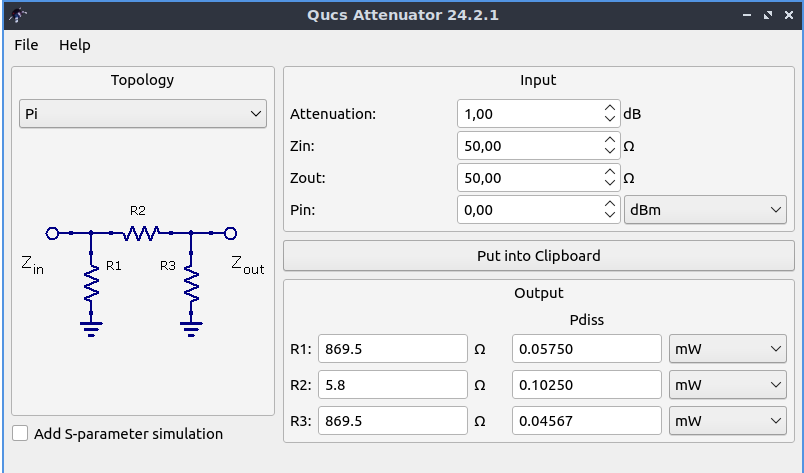
\includegraphics[width=10cm]{/Qucs-S-attenuator-synthesis-GUI.png}
    \caption{Qucs-S attenuator synthesis GUI}
    \label{fig:qucs-s-attenuator-synthesis-GUI}
\end{figure}

%\clearpage
\subsubsection{$\pi$-type attenuator}

\noindent The $\pi$ and T-type attenuators owe their names because to the shape of their layout. Both topologies are easy to implement, provide two-port matching and have broadband response. For these reasons, they are widely used in RF circuit design.

\begin{figure}[ht]
    \centering
    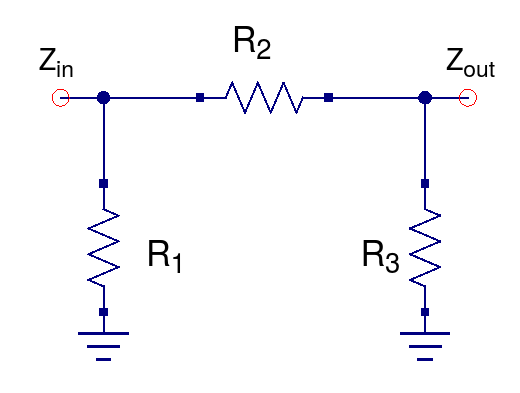
\includegraphics[width=5cm]{pi-attenuator-schematic.png}
    \caption{$\pi$-type attenuator schematic}
    \label{fig:pi-type-attenuator-schematic}
\end{figure}

\noindent The design equations are the following \cite{vizmuller1995rf}:

\begin{equation}
    R_2 = \frac{1}{2} \cdot (10^{\frac{\alpha}{10}} - 1) \cdot \sqrt{\frac{Z_{in} \cdot Z_{out}}{10^{\frac{\alpha}{10}}}}
\end{equation}

\begin{equation}
    R_1 = \frac{1} {\frac{10^{\frac{\alpha}{10}}+1}{Z_{in} \cdot (10^{\frac{\alpha}{10}} - 1)} - \frac{1}{R_2}}
\end{equation}

\begin{equation}
    R_3 = \frac{1} {\frac{10^{\frac{\alpha}{10}}+1}{Z_{out} \cdot (10^{\frac{\alpha}{10}} - 1)} - \frac{1}{R_2}}
\end{equation}


\noindent where $\alpha$ is the attenuation in dB. In both T- and $\pi$-type attenuator topologies the minumum attenuation possible depends on the input impedance $Z_{in}$ and the output impedance $Z_{out}$, as shown in Eq. \ref{eq:min_att_pi}

\begin{equation}
    \alpha_{min} = 20 \cdot log_{10} \left( \sqrt{\frac{Z_{in}}{Z_{out}}} + \sqrt{\frac{Z_{in}}{Z_{out}}-1} \right)
    \label{eq:min_att_pi}
\end{equation}


\noindent Fig. \ref{fig:tee-type-minimum-attenuation} shows the minimum attenuation possible in $\pi$ and T-type attenuators for $Z_{in} / Z_{out}$ ratios up to 10.

\begin{figure}[H]
    \centering
    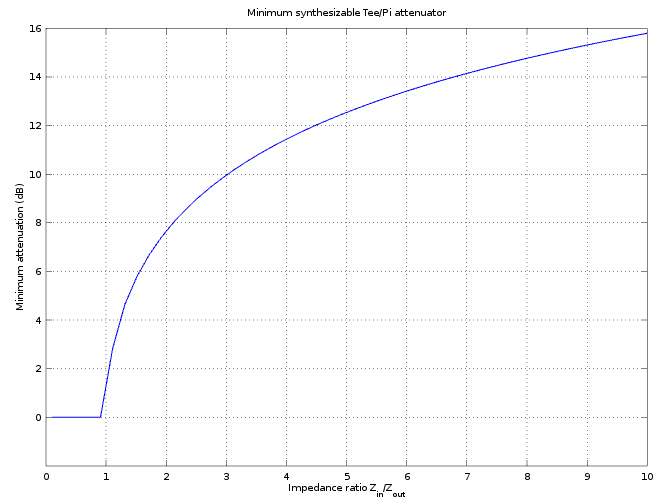
\includegraphics[width=10cm]{pi-tee-minimum-attenuation-vs-Zin-Zout.png}
    \caption{Minimum attenuation possible in T and $\pi$-type attenuators}
    \label{fig:tee-type-minimum-attenuation}
\end{figure}

\noindent The power dissipated in each resistor can be derived using network analysis. Consider the voltages and currents in Fig. \ref{fig:power-dissipation-pi-type-attenuator} and let $P_{R1}$, $P_{R2}$ and $P_{R3}$ be the power dissipated by $R_1$, $R_2$ and $R_3$ respectively. Then:

\begin{figure}[H]
    \centering
    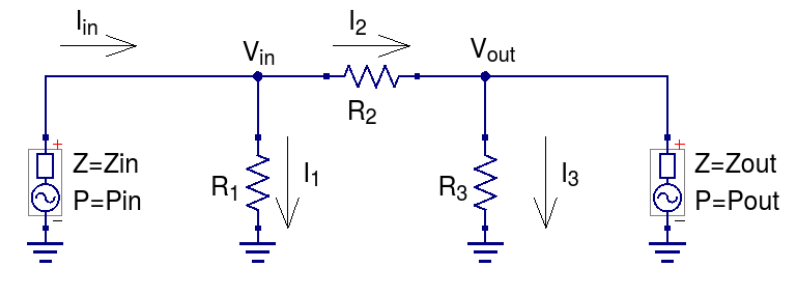
\includegraphics[width=10cm]{pi-attenuator-power-dissipation.png}
    \caption{$\pi$-type attenuator schematic}
    \label{fig:power-dissipation-pi-type-attenuator}
\end{figure}

\begin{equation}
    P_{R1} = P_{in} \cdot \frac{Z_{in}}{R_1}
\end{equation}

\begin{equation}
    P_{R2} = P_{in} \cdot  \frac{R_2 \cdot (R_1 - Z_{in})^2}{R_1^2 \cdot Z_{in}}
\end{equation}

\begin{equation}
    P_{R3} = P_{in} \cdot \frac{\left( R_1 \cdot R_2 - Z_{in} \cdot (R_1 + R_2) \right)^2}{R_1^2 \cdot R_3 \cdot Z_{in}}
\end{equation}

%\clearpage
\subsubsection{T-type attenuator}

\noindent The T-type attenuator (Fig. \ref{fig:tee-type-attenuator-schematic}) is the natural counterpart of the $\pi$-type attenuator. Its design equations can also be found in \cite{vizmuller1995rf}.


\begin{figure}[ht]
    \centering
    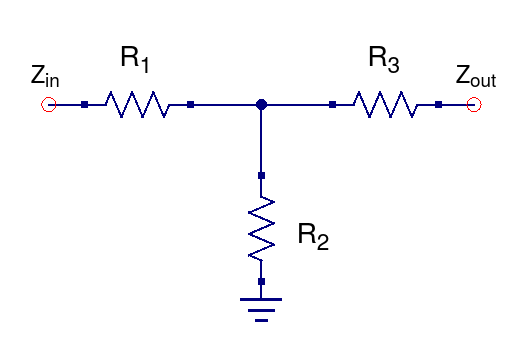
\includegraphics[width=5cm]{tee-attenuator-schematic.png}
    \caption{T-type attenuator}
    \label{fig:tee-type-attenuator-schematic}
\end{figure}

\begin{equation}
    R_{2} = \frac{2 \cdot \sqrt{Z_{in} \cdot Z_{out} \cdot 10^{\alpha/10}}}{10^{\alpha/10}-1}
\end{equation}

\begin{equation}
    R_{1} = \frac{10^{\alpha/10} + 1}{10^{\alpha/10} - 1} \cdot Z_{in} - R_2
\end{equation}

\begin{equation}
    R_{3} = \frac{10^{\alpha/10} + 1}{10^{\alpha/10} - 1} \cdot Z_{out} - R_2
\end{equation}


\noindent where $\alpha$ is the attenuation in dB. The power dissipated in each resistor can be derived using network analysis. Consider the node voltages and currents indicated in Fig. \ref{fig:power-dissipation-tee-type-attenuator} and let $P_{R1}$, $P_{R2}$ and $P_{R3}$ be the power dissipated by $R_1$, $R_2$ and $R_3$, respectively.

\begin{figure}[ht]
    \centering
    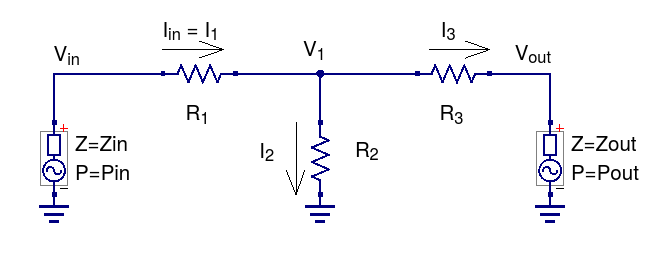
\includegraphics[width=10cm]{tee-attenuator-power-dissipation.png}
    \caption{Node voltages and currents for the T-type attenuator}
    \label{fig:power-dissipation-tee-type-attenuator}
\end{figure}

\noindent Then,

\begin{equation}
    P_{R1} = P_{in} \cdot \frac{R_1}{Z_{in}}
\end{equation}

\begin{equation}
    P_{R2} = P_{in} \cdot  \frac{(R_1 - Z_{in})^2}{R_2 \cdot Z_{in}}
\end{equation}

\begin{equation}
    P_{R3} = P_{in} \cdot \frac{R_3 \cdot (R_1 + R_2 - Z_{in})^2}{Z_{in} \cdot R_2^2}
\end{equation}


\noindent Fig. \ref{fig:pi-tee-relative-power-dissipation-50-Ohm} shows the relative power dissipation per resistance in a $\pi$ and $T$-type attenuators in a 50 $\Omega$ system. As shown, $R_1$ dissipates most of the power for attenuations greater than 6 dB and it dissipates more than the 90 \% of the power for attenuations greater than 27 dB. Please also notice that the power dissipation curves of the $\pi$ and T-type attenuators are the same as long as $Z_{in} = Z_{out}$. However, as shown in Fig. \ref{fig:pi-tee-relative-power-dissipation-50-75-Ohm} if $Z_{in} \neq Z_{out}$ the relative power dissipated at the resistors differs between the $\pi$ and the T-type attenuator.

\begin{figure}[ht]
    \centering
    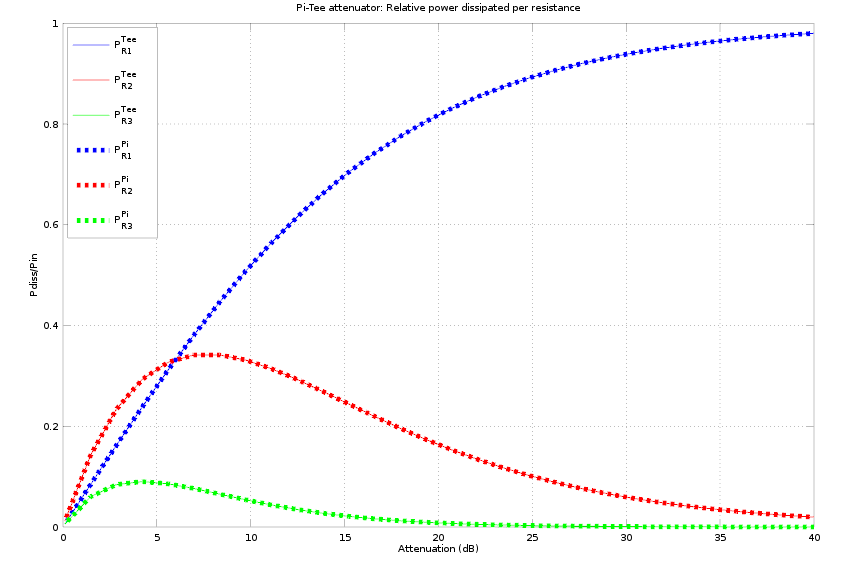
\includegraphics[width=10cm]{pi-tee-relative-power-dissipation-50-Ohm.png}
    \caption{Power dissipated at the resistors in the $\pi$ and T-type attenuators relative to the input power. $Z_{in} = Z_{out} = 50 \Omega$}
    \label{fig:pi-tee-relative-power-dissipation-50-Ohm}
\end{figure}

\begin{figure}[ht]
    \centering
    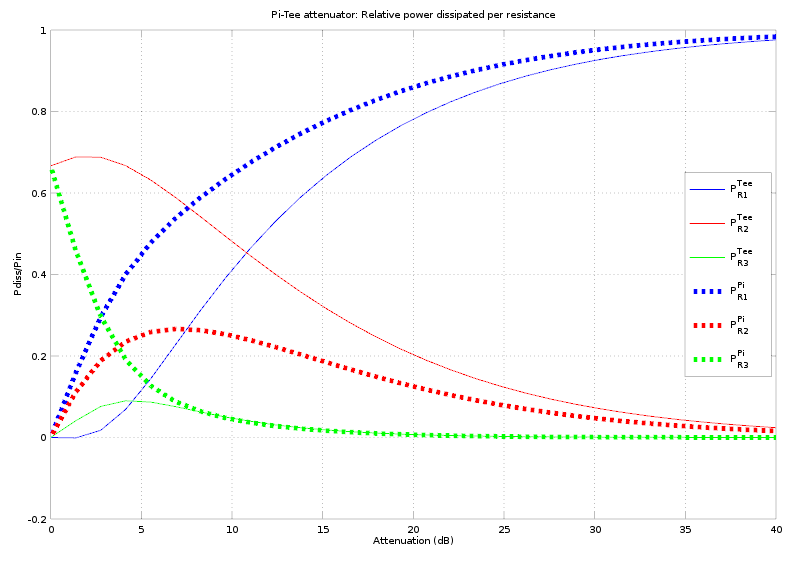
\includegraphics[width=10cm]{pi-tee-relative-power-dissipation-50-75-Ohm.png}
    \caption{Power dissipated in the resistors for the $\pi$ and T-type attenuators with respect to the input power. $Z_{in} = 50 \Omega, Z_{out} = 75 \Omega$}
    \label{fig:pi-tee-relative-power-dissipation-50-75-Ohm}
\end{figure}

%\clearpage
\subsubsection{Bridged-T attenuator}

\noindent The bridged-T attenuator (Fig. \ref{fig:bridged-tee-attenuator-schematic}) requires $Z_{in}$ and $Z_{out}$ to be equal. The design equations are the following \cite{vizmuller1995rf}:

\begin{figure}[ht]
    \centering
    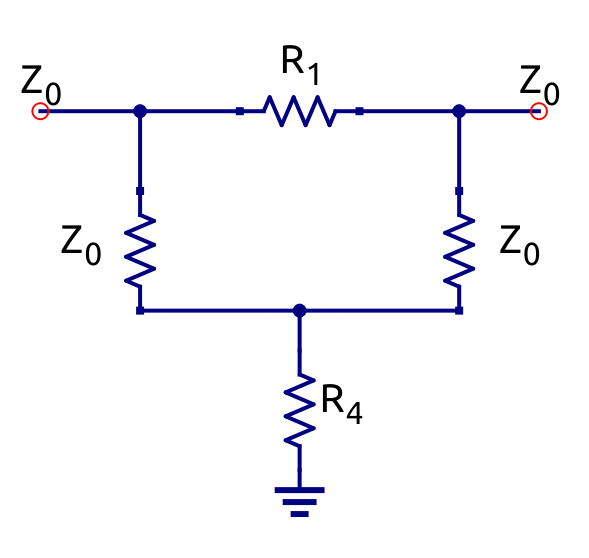
\includegraphics[width=5cm]{bridged-tee-attenuator-schematic.png}
    \caption{Bridged-T attenuator}
    \label{fig:bridged-tee-attenuator-schematic}
\end{figure}

\begin{equation}
    R_1 = Z_0 \cdot (10^{\alpha/20} - 1)
\end{equation}

\begin{equation}
    R_4 = \frac{Z_0}{10^{\alpha/20} - 1}
\end{equation}

\noindent where $\alpha$ is the attenuation in dB. The power dissipation expressions for each resistor are the following:

\begin{equation}
    P_{R1} = P_{in} \cdot \frac{4 \cdot R_1 \cdot R_4^2 \cdot Z_0}{(R_1 \cdot R_4 + Z_0 \cdot (2 \cdot R_4 + Z_0))^2}
\end{equation}

\begin{equation}
    P_{R2} = P_{in} \cdot \frac{(R_1 \cdot R_4 + Z_0^2)^2}{(R_1 \cdot R_4 + Z_0 \cdot (2 \cdot R_4 + Z_0))^2}
\end{equation}

\begin{equation}
    P_{R3} = 0
\end{equation}

\begin{equation}
    P_{R4} = P_{in} \cdot  \frac{4 \cdot R_4 \cdot Z_0^3}{(R_1 \cdot R_4 + Z_0 \cdot (2 \cdot R_4 + Z_0))^2}
\end{equation}

\noindent Fig. \ref{fig:pi-tee-relative-power-dissipation-50-Ohm} shows the power dissipated by each resistor with respect to the input power. Notice that the vast majority of the power is dissipated by $R_2 (= Z_0)$ for attenuations larger than 6 dB.


\begin{figure}[ht]
    \centering
    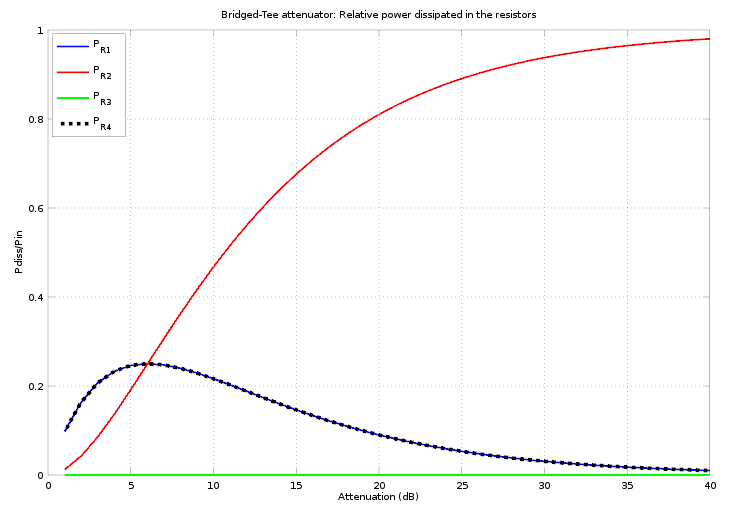
\includegraphics[width=10cm]{bridged-tee-relative-power-dissipation-50-Ohm.png}
    \caption{Power dissipated in the resistor for the bridged-T attenuator with respect to the input power. $Z_{in} = Z_{out} = 50 \Omega$}
    \label{fig:bridged-tee-relative-power-dissipation-50-Ohm}
\end{figure}

%\clearpage
\subsubsection{Reflection attenuator}

\noindent The reflection attenuator \cite{pin_diode_designer_handbook} uses a quadrature hybrid and provides a wideband response and impednace match at the input and output ports.

\begin{figure}[ht]
    \centering
    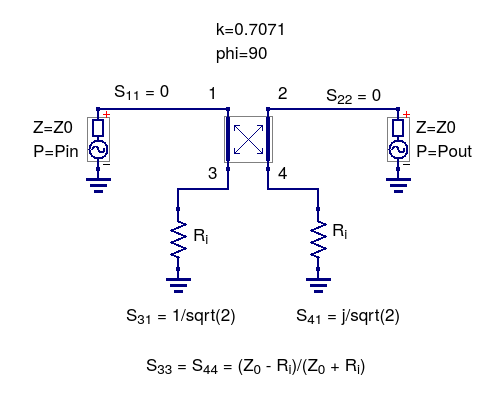
\includegraphics[width=10cm]{reflection-attenuator-schematic.png}
    \caption{Reflection attenuator}
    \label{fig:reflection-attenuator-schematic}
\end{figure}

\noindent The design equations can be obtained from S-parameter analysis.

\begin{equation}
    S_{21} = S_{31} \cdot (-S_{33}) \cdot S_{23} + S_{41} \cdot (-S_{44}) \cdot S_{24} = \left( \frac{Z_0 - R_i}{Z_0 + R_i} \right) \cdot e^{j \cdot \pi/2}
\end{equation}

\noindent Then, the attenuation (in dB) is given by:

\begin{equation}
    \alpha = -20 \cdot log_{10} \left( \lvert S_{21} \rvert \right) = -20 \cdot log_{10} \left( \left| \frac{Z_0 - R_i}{Z_0 + R_i} \right| \right)
    \label{eq:attenuation-eq-reflection-attenuator}
\end{equation}

\noindent Clearing $R_i$ from Eq. \ref{eq:attenuation-eq-reflection-attenuator}:

\begin{equation}
    R_i = \begin{cases} Z_0 \cdot \frac{10^{-\alpha/20} - 1}{10^{-\alpha/20} + 1}, & \text{if  } R_i <  Z_0 \\ Z_0 \cdot \frac{1 + 10^{-\alpha/20}}{1 - 10^{-\alpha/20}}, & \text{if  } R_i > Z_0 \end{cases}
\end{equation}

\noindent The power dissipation equations are derived similarly. Let be $P_{inc}$, $P_{refl}$, and $P_{diss}$ the incident, reflected and dissipated power in a resistor, respectively.

\begin{equation}
    P_{inc}^{R_i} = P_{in} \cdot \lvert S_{i1} \rvert^2
\end{equation}

\begin{equation}
    P_{refl}^{R_i} = P_{in} \cdot \lvert S_{ii} \rvert^2
\end{equation}

\begin{equation}
    P_{diss}^{R_i} = P_{inc}^{R_i} - P_{refl}^{R_i} = P_{in} \cdot \lvert S_{i1} \rvert^2 \cdot (1 - \lvert S_{ii} \rvert^2)
\end{equation}

\noindent Being $S_{ii} = \frac{Z_0 - R_i}{Z_0 + R_i}$ and $S_{i1} = \lvert \frac{1}{\sqrt{2}}\rvert$

\begin{equation}
    P_{diss}^{Ri} = \frac{P_{in}}{2} \cdot \left( 1  - \left| \frac{Z_0 - R_i}{Z_0 + R_i}\right|^2\right)
\end{equation}

\begin{equation}
    P_{diss}^{Ri} = \frac{P_{in}}{2} \cdot \left( 1 - 10^{-\alpha/10}\right)
\end{equation}

\noindent Thus, the power dissipated by the resistors is the same regardless $R_i < Z_0$ or $R_i > Z_0$

\begin{figure}[ht]
    \centering
    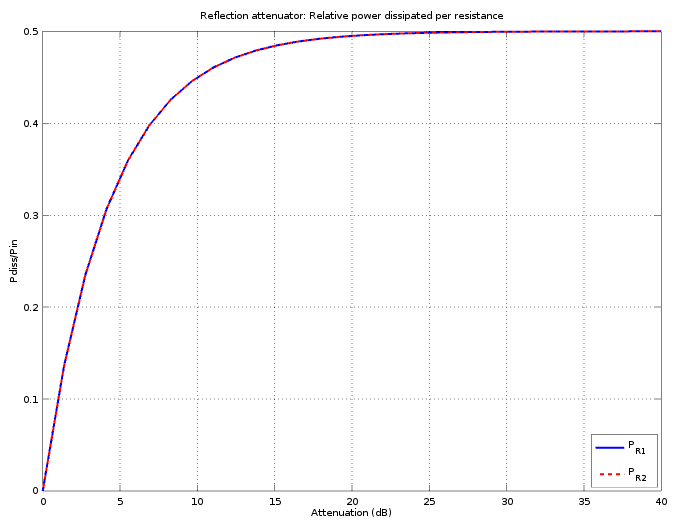
\includegraphics[width=10cm]{reflective-att-relative-power-dissipation-50-Ohm.png}
    \caption{Power dissipated in the resistors in the reflective attenuator relative to the input power. $Z_{in} = Z_{out} = 50 \Omega$}
    \label{fig:reflective-att-relative-power-dissipation-50-Ohm}
\end{figure}
%\clearpage
\subsubsection{Quarter-wavelength series}

\noindent Quarter-wavelength attenuators (both series and shunt arrangements) are microwave attenuators that use a $\lambda/4$ inverter. These types of attenuators only provide matching at the input port \cite{pin_diode_designer_handbook}.

\begin{figure}[ht]
    \centering
    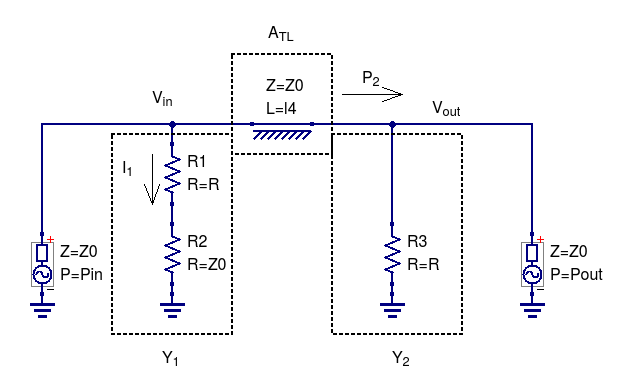
\includegraphics[width=10cm]{qw-series-attenuator-schematic.png}
    \caption{Quarter wavelength series attenuator}
    \label{fig:qw-series-attenuator-schematic}
\end{figure}

\noindent The design equations of the quarter-wavelength series attenuator can be derived using cascade analysis:

\begin{equation}
    Y_1 = \begin{pmatrix}
        1 & 0\\
        \frac{1}{R + Z_0} & 1
    \end{pmatrix}
\end{equation}

\begin{equation}
    A_{TL} = \begin{pmatrix}
        cosh(\gamma \cdot l) & Z_0 \cdot sinh(\gamma \cdot l)\\
        \frac{1}{Z_0} \cdot sinh(\gamma \cdot l)  & cosh(\gamma \cdot l)
    \end{pmatrix}
\end{equation}

\noindent where $\gamma = \alpha + j \cdot \beta$ is the propagation constant. Since the $\lambda/4$ transmission line is supposed to be lossless, then $\gamma = j \cdot \beta = j \cdot \frac{2 \cdot \pi}{\lambda}$ and, consequently:

\begin{equation}
    A_{TL} = \begin{pmatrix}
        0 & j \cdot Z_0\\
        \frac{j}{Z_0}  & 0
    \end{pmatrix}
\end{equation}

\noindent The ABCD matrix of the $Y_2$ block is simply:

\begin{equation}
    Y_{2} = \begin{pmatrix}
        1 & 0\\
        \frac{1}{R}  & 1
    \end{pmatrix}
\end{equation}

\noindent The overall ABCD matrix is given by:

\begin{equation}
    A_{QW_{series}} = Y_1 \cdot A_{TL} \cdot Y_2 = j \cdot Z_0 \cdot \begin{pmatrix}
        \frac{1}{R} & 1\\
        \left( \frac{1}{R \cdot (R + Z_0)} + \frac{1}{Z_0^2} \right)  & \frac{1}{R + Z_0}
    \end{pmatrix}
\end{equation}

\noindent Using the conversion formulae between ABCD and S parameters \cite{pozar2012microwave}:

\begin{equation}
    S = \begin{pmatrix}
        0 & -j \cdot \frac{R}{R + Z_0}\\
        -j \cdot \frac{R}{R+Z_0}  & \frac{Z_0^2}{(R + Z_0)^2}
    \end{pmatrix}
\end{equation}

\noindent Thus, the attenuation (in dB) can be expressed in terms of R and $Z_0$ as follows:

\begin{equation}
    \alpha = -20 \cdot log_{10} \left( \frac{R}{R+Z_0}\right)
\end{equation}

\noindent Then,

\begin{equation}
    R = \frac{Z_0}{10^{\frac{\alpha}{20}} - 1}
\end{equation}

\noindent The impedance inversion property of the $\lambda$/4-transmission line holds in the vecinity of the center frequency. The general (broadband) expressions for the S-parameters of the quarter wavelength attenuators are much more complex and numeric S-parameter simulation analysis is more convenient for the analysis.

\noindent The impedance seen at the output port is given by:

\begin{equation}
    Z_{out} = \frac{R^2 \cdot Z_0 + 2 \cdot R \cdot Z_0^2}{R^2 + 2 \cdot R \cdot Z_0 + 2 \cdot Z_0^2}
\end{equation}

\noindent The power dissipated in the resistors at the center frequency ($f_c$) is calculated as follows:

\begin{equation}
    P_{R1} = P_{R3} = I_1^2 \cdot R_1 = \left( \frac{V_{in}}{R_1 + Z_0}\right)^2 \cdot R_1= P_{in} \cdot \left( \frac{ Z_0}{(R_1 + Z_0)^2} \right) \cdot R_1
\end{equation}

\begin{equation}
    P_{R2} = P_{in} \cdot \left( \frac{Z_0}{R_1 + Z_0} \right)^2
\end{equation}

\begin{figure}[ht]
    \centering
    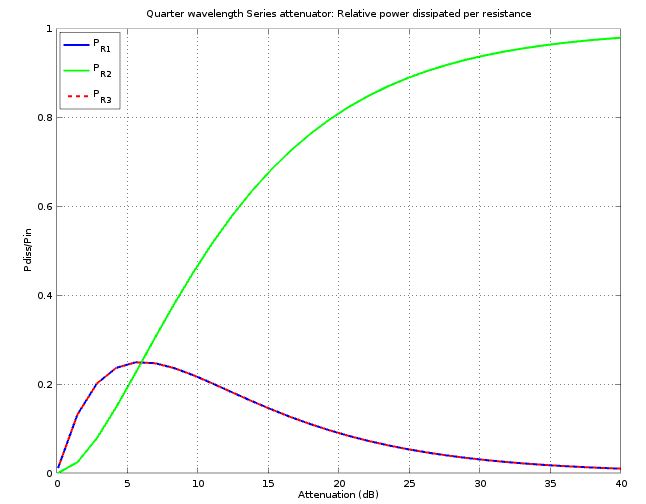
\includegraphics[width=10cm]{qw-series-relative-power-dissipation-50-Ohm.png}
    \caption{Power dissipated in the resistors of the quarter wavelength series attenuator with respect to the input power. $Z_{in} = Z_{out} = 50 \Omega$}
    \label{fig:qw-series-att-relative-power-dissipation-50-Ohm}
\end{figure}
%\clearpage
\subsubsection{Quarter-wavelength shunt}

\begin{figure}[ht]
    \centering
    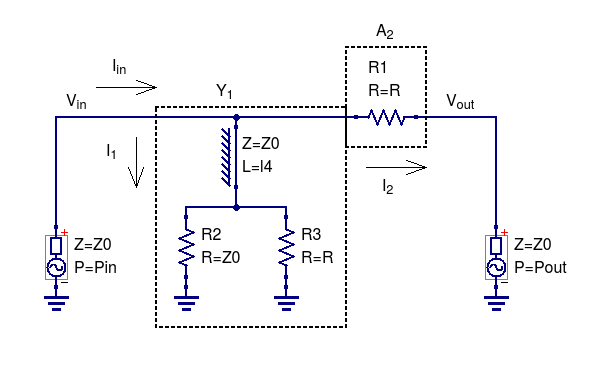
\includegraphics[width=10cm]{qw-shunt-attenuator-schematic.png}
    \caption{Quarter wavelength shunt attenuator}
    \label{fig:qw-shunt-attenuator-schematic}
\end{figure}

\noindent At the center frequency, the $\lambda/4$ transmission line behaves as an impedance inverter and its input impedance is given by:

\begin{equation}
    Z_{TL} = \frac{Z_0^2}{Z_L}, Z_L = \frac{R \cdot Z_0}{R + Z_0} \Rightarrow Z_{TL} = Z_0 \cdot \frac{R + Z_0}{R}
\end{equation}

\noindent The ABCD parameters of the shunt branch ($Y_2$) are the following:

\begin{equation}
    Y_1 = \begin{pmatrix}
        1 & 0\\
        \frac{R}{Z_0 \cdot (R+Z_0)}  & 1
    \end{pmatrix}
\end{equation}

\noindent The ABCD parameters of the series resistor is:
\begin{equation}
    A_2 = \begin{pmatrix}
        1 & R\\
        0  & 1
    \end{pmatrix}
\end{equation}

\noindent Therefore, the ABCD parameters of the whole quarter-wavelength attenuator is simply the product of $Y_1$ and $A_2$:

\begin{equation}
    A_{qw_{shunt}} = Y_1 \cdot A_1 = \begin{pmatrix}
        1 & R\\
        \frac{R}{Z_0 \cdot(R+Z_0)}  & 1 + \frac{R^2}{Z_0 \cdot(R+Z_0)}
    \end{pmatrix}
\end{equation}

\noindent Using the conversion formulae between ABCD and S parameters \cite{pozar2012microwave}:
\begin{equation}
    S_{qw_{shunt}} = \begin{pmatrix}
        0 & \frac{Z_0}{R + Z_0}\\
        \frac{Z_0}{R+Z_0}  & \frac{R^2}{(R+Z_0)^2}
    \end{pmatrix}
\end{equation}

\noindent and the attenuation (in dB) is obtained in terms of R and $Z_0$ as:

\begin{equation}
    \alpha = -20 \cdot log_{10} \left( \frac{Z_0}{R + Z_0}\right)
\end{equation}

\noindent Thus, the resistor value is determined by the attenuation and the system impedance as:

\begin{equation}
    R = Z_0 \cdot \left( 10^{\frac{\alpha}{20}} - 1 \right)
\end{equation}

\noindent and the output impedance is:

\begin{equation}
    Z_{out} = R + Z_1 \parallel Z_0 = R + \frac{Z_0 \cdot (R + Z_0)}{2 \cdot R + Z_0}
\end{equation}

\noindent Concerning power dissipation, the power dissipated in the shunt branch is:

\begin{equation}
    P_{shunt} = \frac{V_{in}^2}{Z_{TL}} = P_{in} \cdot \frac{R}{R+Z_0}
\end{equation}

\noindent The voltage at the node between the transmission line and the shunt resistors may be expressed as:

\begin{equation}
    V_{1} = \sqrt{P_{shunt} \cdot R_{eq}} = R \cdot \frac{\sqrt{P_{in} \cdot Z_0}}{R + Z_0}
\end{equation}

\noindent Thus, the power dissipated in $R_2$ and $R_3$ is given by:

\begin{equation}
    P_{R2} = P_{in} \cdot \frac{R^2}{(R + Z_0)^2}
\end{equation}

\begin{equation}
    P_{R3} = P_{in} \cdot \frac{R \cdot Z_0}{(R + Z_0)^2}
\end{equation}

\noindent Being $I_1 = \frac{V_{in}}{Z_{TL}}$ the current flowing through the shunt branch and $I_{in} = \sqrt{\frac{P_{in}}{Z_{TL}}}$ the current delivered by the source, the current through $R_1$ and the load is $I_2 = I_{in} - I_1$ and, consequently, the power dissipated in $R_1$ is:

\begin{equation}
    P_{R1} = P_{in} \cdot \frac {R \cdot Z_0}{(R+Z_0)^2}
\end{equation}
%\clearpage
\subsubsection{L-pad ($1^{st}$ series)}

\noindent L-pad resistive networks are typically used for very broadband impedance matching in applications where a significant amount of insertion loss can be accepted (e.g. 50 $\Omega$ to 75 $\Omega$ matching pads).

\begin{figure}[ht]
    \centering
    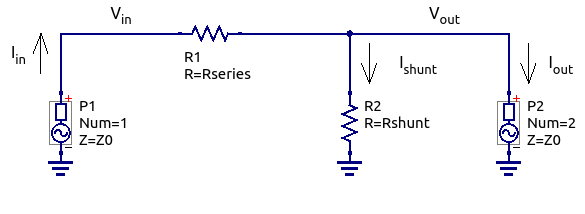
\includegraphics[width=10cm]{l-pad-series-attenuator-schematic.png}
    \caption{L-pad series attenuator}
    \label{fig:l-pad-series-attenuator-schematic}
\end{figure}

\noindent As before, the design equations can be obtained through network analysis. Being $I_{in} = I_{shunt} + I_{out}$. Provided that:

\begin{equation}
    \begin{cases} I_{shunt} = \frac{Vout}{R_{shunt}} \\ I_{in} = - \frac{V_{in}}{Z_0} \\ I_{out} = \frac{V_{out}}{Z_0} \end{cases}
\end{equation}

\noindent Combining these equations into the first one, we get that the voltage gain is:

\begin{equation}
    A_v = \frac{V_{out}}{V_{in}} = -\frac{R_{shunt}}{Z_0 + R_{shunt}}
\end{equation}

\noindent Provided that the attenuation (in natural units) is related to the voltage gain as $\alpha^{n.u.} = A_v^2$, the following expression holds:

\begin{equation}
    (1 - \alpha^{n.u.}) \cdot R_{shunt}^2 - 2 \cdot \alpha^{n.u.} \cdot Z_0 \cdot R_{shunt} - \alpha \cdot Z_0 = 0
    \label{eq:L-pad-series-equation}
\end{equation}

\noindent Eq. \ref{eq:L-pad-series-equation} has two solutions:

\begin{equation}
    \begin{cases}
        R_{shunt}^{S1} = \frac{- Z_0 \cdot (\alpha^{n.u.} + \sqrt{\alpha^{n.u.}})}{\alpha^{n.u.} - 1} & \text{Solution 1} \\
        R_{shunt}^{S2} = \frac{- Z_0 \cdot (\alpha^{n.u.} - \sqrt{\alpha^{n.u.}})}{\alpha^{n.u.} - 1} & \text{Solution 2}
    \end{cases}
\end{equation}

\noindent A valid solution must also satisfy the input match condition:

\begin{equation}
    Z_0 = R_{series} + R_{shunt} \parallel Z_{load} \Rightarrow R_{series} = \frac{Z_0^2}{Z_0 + R_{shunt}}
\end{equation}

\noindent Each solution for $R_{shunt}$ is related to a $R_{series}$ value:

\begin{equation}
    \begin{cases}
        R_{series}^{S1} = -Z_0 \cdot \frac{\alpha^{n.u.} - 1}{\sqrt{\alpha^{n.u.}} + 1}  & \text{Solution 1} \\
        R_{series}^{S2} = Z_0 \cdot \frac{\alpha^{n.u.} - 1}{\sqrt{\alpha^{n.u.}} - 1} & \text{Solution 2}
    \end{cases}
\end{equation}

\noindent Provided that $\alpha^{n.u.} < 1$, Solution 1 is always valid since $R_{shunt}, R_{series} > 0$. Solution 2 yields negative resistor values.

\noindent The output impedance of the L-pad can be obtained as follows:

\begin{equation}
    Z_{out} = R_{shunt} \parallel \left( R_{series} + Z_0 \right) = \frac{R_{shunt} \cdot \left( R_{series} + Z_0 \right)}{R_{shunt} + R_{series} + Z_0}
\end{equation}

\noindent Concerning power dissipation in the resistors, the following expressions were obtained:

\begin{equation}
    P_{diss}^{R_{series}} = P_{in} \cdot \left( 1 - \sqrt{\alpha^{n.u.}} \right)
\end{equation}

\begin{equation}
    P_{diss}^{R_{shunt}} = P_{in} \cdot \alpha^{n.u.} \frac{1 - \alpha^{n.u.}}{\alpha^{n.u.} + \sqrt{\alpha^{n.u.}}}
\end{equation}
%\clearpage
\subsubsection{L-pad ($1^{st}$ shunt)}

\noindent The schematic of the L-pad $1^{st}$ shunt attenuator is shown in Fig. \ref{fig:l-pad-shunt-attenuator-schematic} and its design equations are derived as follows using basic network analysis:

\begin{figure}[ht]
    \centering
    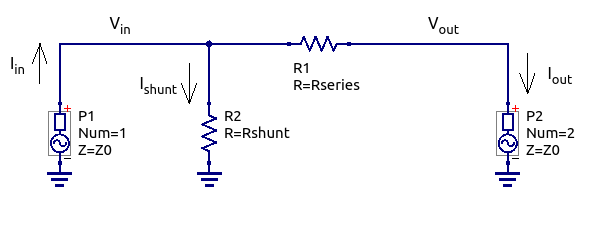
\includegraphics[width=10cm]{l-pad-shunt-attenuator-schematic.png}
    \caption{L-pad shunt attenuator}
    \label{fig:l-pad-shunt-attenuator-schematic}
\end{figure}

\begin{equation}
    \frac{V_{in} - V_{out}}{R_{series}} = \frac{V_{out}}{Z_0} \Rightarrow A_v = \sqrt{\alpha^{n.u.}} = \frac{V_{out}}{V_{in}} = \frac{Z_0}{Z_0 + R_{series}}
\end{equation}

\noindent Consequently,

\begin{equation}
    R_{series} = Z_0 \cdot \frac{1 - \sqrt{\alpha^{n.u.}}}{\sqrt{\alpha^{n.u.}}}
\end{equation}

\noindent The input port must be matched to $Z_0$, so:

\begin{equation}
    Z_0 = R_{shunt} \parallel R_{series} + Z_0 \Rightarrow R_{shunt} = Z_0 \cdot \frac{1}{1 - \sqrt{\alpha^{n.u.}}}
\end{equation}

\noindent The output impedance of the L-pad is, then:

\begin{equation}
    Z_{out} = R_{series} + R_{shunt} \parallel Z_0 = - Z_0 \cdot \frac{\alpha^{n.u.} - 2 \cdot \sqrt{\alpha^{n.u.}} + 2}{\alpha^{n.u.} - 2 \cdot \sqrt{\alpha^{n.u.}}}
\end{equation}

\noindent Concerning the power dissipation in the resistors, the corresponding equations for the shunt and the series resistors were found to be:

\begin{equation}
    P_{diss}^{shunt} = P_{in} \cdot \left( 1 - \sqrt{\alpha^{n.u.}}\right)
\end{equation}

\begin{equation}
    P_{diss}^{series} = P_{in} \cdot \sqrt{\alpha^{n.u.}} \cdot \frac{1 - 2 \cdot \sqrt{\alpha^{n.u.}} + \alpha}{1 - \sqrt{\alpha^{n.u.}}}
\end{equation}


%\clearpage
\subsubsection{Series resistor}

\noindent Single resistor attenuators are unmatched at both the input and the output ports and they are may be found in applications where impedance match is not required. They can be used as broadband lossy matching networks as well.

\begin{figure}[ht]
    \centering
    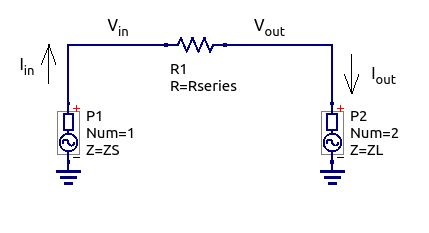
\includegraphics[width=10cm]{r-series-attenuator-schematic.png}
    \caption{Series resistor attenuator}
    \label{fig:r-series-attenuator-schematic}
\end{figure}

\noindent The design equations are derived more easily from the point of view of the power reflection and transmission rather than from the nodal analysis perspective. There are two interfaces where the impedance mismatch ocurr: the first one between the source and the series resistor and the second one between the series resistor and the load impedance.

\noindent In the interface between the source impedance and the resistor, the loss caused by the mismatch is given by:

\begin{equation}
    t_1 = 1 - \left| \frac{Z_S - (R + Z_L)}{Z_S + R + Z_L}\right|
\end{equation}

\noindent Between the resistor and the load impendance, the loss caused by the mismatch is:

\begin{equation}
    t_2 = 1 - \left| \frac{(Z_S + R) - Z_L}{Z_S + R + Z_L}\right|
\end{equation}

\noindent Consequently, the total power loss is:

\begin{equation}
    t = t_1 \cdot t_2 = \frac{4 \cdot Z_L \cdot Z_S}{R^2 + 2 \cdot R \cdot Z_L + Z_L^2 + 2 \cdot Z_S \cdot (R  + Z_L) + Z_S^2}
    \label{eq:r-series-power-loss}
\end{equation}

\noindent Eq. \ref{eq:r-series-power-loss} gives two solutions, but only one gives positive values:

\begin{equation}
    R = \frac{1}{\alpha^{n.u.}} \cdot \left( -\alpha^{n.u.} \cdot (Z_L + Z_S) + 2 \sqrt{Z_L \cdot Z_S \cdot \alpha^{n.u.}} \right)
\end{equation}
%\clearpage
\subsubsection{Shunt resistor}

\begin{figure}[ht]
    \centering
    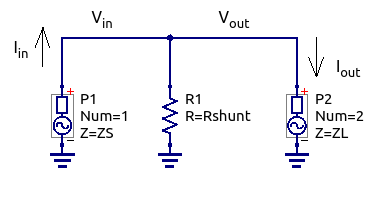
\includegraphics[width=10cm]{r-shunt-attenuator-schematic.png}
    \caption{Shunt resistor attenuator}
    \label{fig:r-shunt-attenuator-schematic}
\end{figure}

\noindent As in the case of the series resistor attenuator, the design equations can be derived from the loss caused by the impedance mismatch in the input and the output interfaces. Between the source impedance and the shunt resistor, the mismatch was found to be:

\begin{equation}
    t_1 = 1 - \left| \frac{Z_S - R \parallel Z_L}{Z_S + R \parallel Z_L} \right|
\end{equation}

\noindent Similarly, between the shunt resistor and the load impedance, the mismatch causes a insertion loss of:

\begin{equation}
    t_2 = 1 - \left| \frac{Z_S \parallel R - Z_L}{Z_S \parallel R + Z_L} \right|
\end{equation}

\noindent Consequently, the overall power loss is:

\begin{equation}
    t = t_1 \cdot t_2 = \frac{4 \cdot R^2 \cdot Z_S \cdot Z_L}{R^2 \cdot Z_L^2 + Z_S^2 \cdot (R^2 + 2 \cdot R \cdot Z_L + Z_L^2) + 2 \cdot Z_S \cdot Z_L \cdot R \cdot (R  + Z_L)}
    \label{eq:r-shunt-power-loss}
\end{equation}

\noindent As before, Eq. \ref{eq:r-shunt-power-loss} gives two solutions, but only one gives positive resistor values:

\begin{equation}
    R = Z_S \cdot Z_L \cdot \frac{2 \cdot \sqrt{Z_S \cdot Z_L \cdot \alpha^{n.u.}} + \alpha^{n.u.}  \cdot \left( Z_L + Z_S\right)}{4 \cdot Z_S \cdot Z_L - \alpha^{n.u.} \cdot (Z_L^2 + 2 \cdot Z_L \cdot Z_S + Z_S^2)}
\end{equation}
\endinput

